\chapter{Graphs and Network Formation}
\label{chp:graphTheory} 

In nature and society, many scenarios can be described using graphs. Infrastructure, such as railroads, water pipelines and electricity grid, societal relationships and disease epidemics, can all be visualized using graphs. Cyber-insurance is no exception, and can also be structured as a graph. This is of interest because, when one can describe a phenomenon with graphs, it is easier to analyze and possibly find some characteristics, hence the graph can be used as an analytic tool \cite{audestad}. 

Several studies have been done on the characteristics of different graphs, such as E-R graphs and A-B graphs (scale-free graphs), these are thoroughly described in the methodology chapter of this thesis. In addition, one has found special characteristics of star-shaped graphs and cliques. This chapter will highlight which characteristics that are desirable in the cyber-insurance market, and which structures that possess these characteristics. These findings will serve as the foundation of our models, where we try to force these graph structures to emerge.
 
\section{Real-world graph structures}
As a starting point, let's have a look at a couple of real-world examples of how complex systems with huge amount of data could be structured as graphs. We will see how complex structures become rather intuitive when presented as graphs. By looking at the graph structure, one can determine what type of graph that appears, and hence certain characteristics will apply.  

\subparagraph{Stock markets.} The research paper \cite{greekStockMarket} analyzes the correlation between different stocks in the Greek stock market in year 1997. The authors compared the daily closing price of stock $i$ at day $t$, and compared the similarity of a pair of stocks $i$ and $j$ by using the correlation coefficient. The idea is that the correlation coefficient between a pair of stocks can be expressed using different distances in a graph structure. A short distance means high correlation and a long distance means low correlation between the stocks. Normally, this network would be shown as a fully connected graph, which will consist of $\frac{n(n-1)}{2}$ edges, and would be difficult to analyze. However, the new approach presents a clear and understandable graph, consisting of $(n-1)$ edges showing the correlations between the stocks.

The resulting graph can be seen in Figure \ref{fig:greekStockMarket}, and shows a network consisting of several clusters linked together. Instead of having to analyze a complex system with huge amounts of data, the stock market can be analyzed by its topological properties, such as the high clustering coefficient, i.e a scale free topology, which will among other things point out which stocks have the most influence on others. 
\begin{figure}[h]
\centering
\begin{tabular}{@{}c@{}}
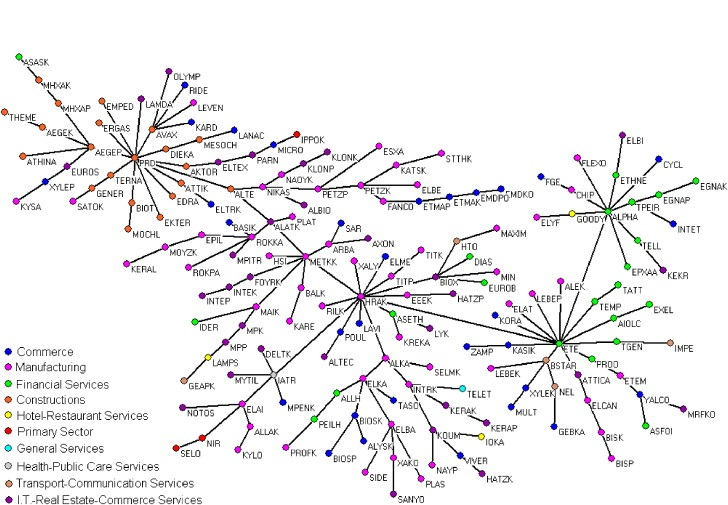
\includegraphics[width=1.0\textwidth]{../Figures/greekStockMarket.jpg}
\end{tabular}
\caption[Network of two stocks' correlation coefficient at Athens Stock Exchange, ASE.]{Network obtained by comparing two stocks' correlation coefficient in the Greek stock market (Athens Stock Exchange, ASE) in year 1997. The different colors represent the different sectors of economic activity \cite{greekStockMarket}.
\label{fig:greekStockMarket}}
\end{figure}

\subparagraph{Airline routes.}
Another real-world network which shows the same characteristics as scale-free graphs is the map of airline routes. Figure \ref{fig:airlineRouteMap} shows the US route map of the American airline company SkyWest. The characteristic clustering emerges in the figure, where a majority of the flights departing from either Denver, Chicago or San Francisco. Not surprisingly, these airports are all in the top 7 busiest airports in the US \cite{busiestAirports}, and serve as hubs for many of SkyWest's flights. In the airline industry some airports are called hubs, because that's what they are, - a connection point for major parts of the network of flights. The network of flights, as depicted in Figure \ref{fig:airlineRouteMap}, follows the characteristics of A-B graphs. Hence, as we can confirm from looking at the graph, the network are vulnerable against direct attacks, meaning that shutting down a low degree airport wont create much trouble. However, if one of the hubs is forced to close, it will provoke huge delays throughout the whole network, because a majority of the destinations is interconnected via the hubs. 


\begin{figure}[h]
\centering
\begin{tabular}{@{}c@{}}
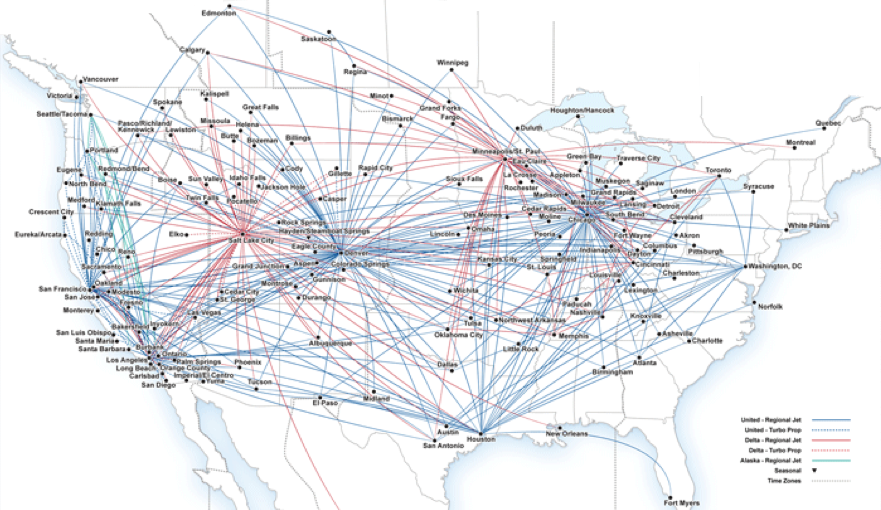
\includegraphics[width=1.0\textwidth]{../Figures/airlineRoutesUSA.png}
\end{tabular}
\caption[SkyWest Airline's combindes route map]{SkyWest Airline's combined route map \cite{airlineRoutes}.
\label{fig:airlineRouteMap}}
\end{figure}

Here, both examples can be characterized as scale-free networks, and the work done by Albert and Barabási shows that a large part of natural systems is in fact scale-free graphs \cite{audestad}. Since we are able to determine the graph's type, which in this case is a scale-free graph, we now know that the graph is vulnerable to attacks directed towards the hubs, i.e. the hubs need to be secured. For example, if a delay occurs at an airline hub, these delays will probably cascade throughout the network.
This shows the strength of being able to structure systems as graphs. When certain structures appear, one can assume that the network will behave according to a set of rules. This is why we wish to determine whether there are any structures that possess preferred characteristics for cyber-insurance, and then find a proper way to force these formations to evolve.


\chapter{Evolutionary dynamics on graphs}
\label{chp:nature} 


In our paper an insurable topology, is an network structure which makes it feasible for both the
 insurer(supply side)  to offer and the customer(demand side) to acquire insurance.
 For this to be possible there are many  difficulties to overcome,  since risks are correlated, 
 one problem is for the insurer to be able to calculate the overall probability of casualty/infection.
 The paper \cite{lieberman2005evolutionary} is about evolutionary dynamics and how certain structures
can amplify or sustain evolution or drift. This is very usefull for our study of insurable topology, if one
can determine some structures, where certain nodes have certain properties, and these structures
then will sustain viruses from spreading, or amplify the incentive for obtaining cyberinsurance and
antivirus, then we can possibly determine if it is an insurable topology.

In the \cite{lieberman2005evolutionary} paper, they show that advantageous mutant inserted in to a
 circulation graph, will have a fixation probability equal to
\begin{equation}  p_{1}=\frac{(1-1/r)}{(1-1/r^{N})} \label{eq:fixation} \end{equation}
A circulation graph is a graph that satisfy these two properties:
\begin{enumerate}
\item the sum of all edges leaving a vertex is equal for all vertexes
\item the sum of all edges entering a vertex i equal for all vertexes
\end{enumerate}
The fixation probability determines how probable it is that the whole network will eventually be
"infected" by the mutant. I.e. it determines the rate of evolution, which relies on both the size of the
network and the evolution speed. 
A probability equal to one means that every node in the network eventually will be affected by the mutant.

The important question that this paper answer, is if it is possible to find graphs with fixation probability that exceeds \ref{eq:fixation}?, and if so, is it possible to suppress drift and amplify selection or visa versa?
\begin{figure}
\centering
\begin{tabular}{@{}c@{}}

\includegraphics[width=0.5\textwidth]{NetworkTopology-Star.png}
\end{tabular}
\caption{\label{fig:star} A star-topology \cite{lieberman2005evolutionary}. }
\end{figure}

The paper shows that in certain graphs this is possible, one example is the star topology \ref{fig:star}.
In this topology the fixation probability is\begin{equation}p_{2}=\frac{(1-1/r^{2})}{(1-1/r^{2N})} \label{eq:fixation2} \end{equation}.
or more generally: \begin{equation}
p_{k}=\frac{(1-1/r^{k})}{(1-1/r^{kN})} \label{eq:fixationk}
\end{equation}
And as we see when comparing \ref{eq:fixation} and \ref{eq:fixation2} the selective difference is
 amplified from $r$ to $r^{2}$, i.e. a star act as an evolutionary amplifier, favoring advantageous
  mutants and inhibiting disadvantageous mutants.
  
When applying this to our scenario, cyber insurance and insurable topologies, we can use this to show
 that if the center node is strongly secured, then the virus will be considered as disadvantageous and
it will be inhibited from fixation with a certain probability. 
This makes the overall risk easier to calculate for both the insurer and the nodes,
and makes it possible and easier to calculate fair and affordable premiums. 
It can also be used as an incentive for the center node to buy insurance or security software, 
because it can easily be shown how probable an infection will occur. 

One could for example force the center node to buy sufficient anti virus, 
by informing it about how likely it will be infected, and how expensive the cyber insurance will be if 
it do not invest sufficiently in self protection. This will make the whole network more secure, 
and the insurer can now offer insurance to the leaf nodes for a fair price with a calculable risk. 
This could also be used to show how information about cyber-insurance or protection software will
spread throughout a network, and if the information is advantageous, eventually all nodes will acquire
the insurance or software.
    
There are other graphs where the fixation probability is equal to \ref{eq:fixationk}, funnel and
metafunnel. And as we know from the (Kapittel om scale-free and naturlige nettverk) there are many
toplogies in our society that are similar to these graphs.  In all of these, it can be
shown that if N is large enough, the fixation probability for advantageous mutant converges to 1, 
and for disadvantageous converges to 0.

\subsection{Network games}
In the paper \cite{networkgames} they show how network games evolve when the payoffs are determined not only by your own decisions, but also by your neighbours. 
A game that is applicable to our scenario is when considering security software, 
security software can be considered as a public good, it suffers from strategic substitutes, i.e. 
that if your neighbour acquire it, it gives you less incentive to also acquiring the software. 
Public goods and security also benefits from positive externalities, when one acquires the software, 
all the neighbours benefits from it, because the risk of being infected decreases.
Lets consider a simple game shown in this paper.
We have an action space: $X=\{0,1\}$, where 1 can be considered as acquiring information, take vaccine, buy security software etc. And 0 is not doing so.
Each node $i$ has a set of neighbours: $N_{i} $ and a payoff function $y_{i}=x_{i}+\bar{x}N_{i}$
The gross payoff of the game is 1 if $y_{i}>=1$ and 0 otherwise. There is a cost of choosing the action 1, and the cost is: $0<c<1$.
%% [location]h-here, t top, b bottom.
\begin{figure}[h]
\centering
\begin{subfigure}{.4\textwidth}
  \centering
  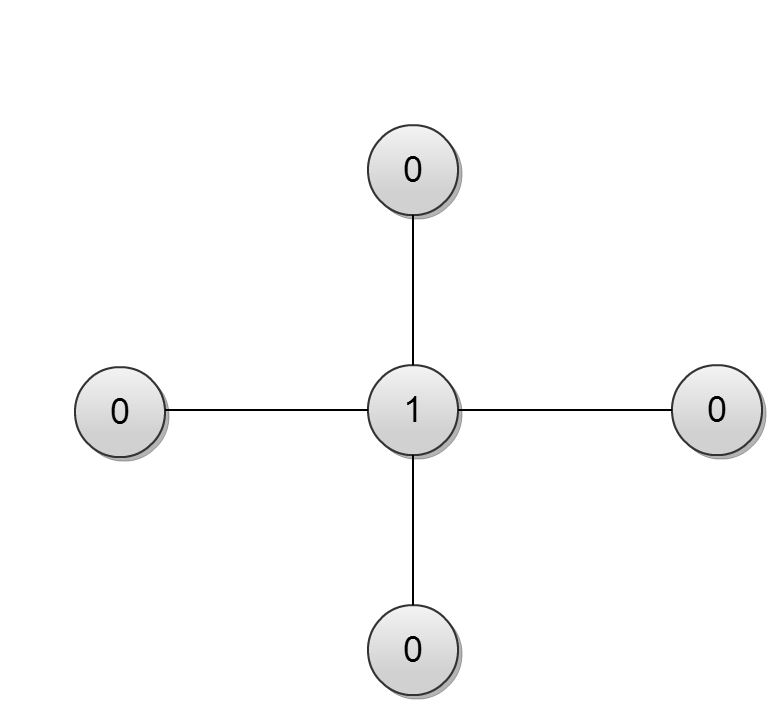
\includegraphics[width=0.8\linewidth]{optimalequilibrium.png}
  \caption{\label{fig:optequi} Socially Optimal equilibrium, center node choose action 1}
\end{subfigure}
\quad
\begin{subfigure}{.4\textwidth}
  \centering
  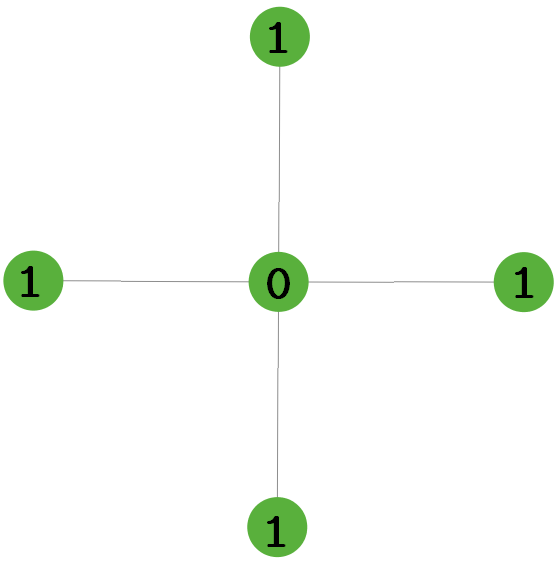
\includegraphics[width=0.8\linewidth]{notoptimalequilibrium.png}
  \caption{\label{fig:notoptequi} Non Socially Optimal equilibrium, leaf nodes choose action 1}
\end{subfigure}
\caption{\label{fig:starequi} Figure \ref{fig:optequi} shows the socially optimal equilibrium, and \ref{fig:notoptequi} shows the non optimal equilibrium.}

\end{figure}

 When we look at the star example, we easily see that there is two equilibriums \ref{fig:starequi}, one where the center node choose action 1 and the rest of the nodes choose action 0, and a second equilibrium where all the leaf nodes chooses 1 and the center choose 0.
The overall payoff in these two differ from each other, the latter is not socially optimal because it
 suffers from a cost equal to: $\#leaf nodes*c$ versus the first equilibrium where the total cost is only $c$.
If we could have forced to network game to end up in the socially optimal equilibrium, this would have been optimal. 
One possibility could be for the insurer to offer cheap insurance to all the leaf nodes, and a expensive one to the center node. By expensive we mean a cost that exceeds the cost of acquiring self protection, because then a rational center node would striclty prefer buying security software, as long as the price for acquiring and maintaining it is less than the possible cost of loss.
\begin{equation}
 U_{center}=-Probability_{casualty}*\alpha-Cost_{selfprotection}
 \label{eq:utility}
 \end{equation} 
A risk averse player would like to maximize her expected utility \ref{eq:utility}. We assume that the probability of casualty is significantly smaller when acquiring self protection, versus not acquiring. If the options for a player is
 either to remove the expected loss of casualty by acquiring self protection, or by insuring against it,
and the expected utility of acquiring insurance is lower than the expected utility of acquiring self protection. The player would strictly prefer self protection. 
This is one possible way of forcing the network game to end up in an insurable star topology.
//
Thoughts on what this fixes in a simple way...
The insurer can now calculate the probability for catastrophic event(all nodes suffer), and now atleast has a measurement on the correlated risk. It has also limited the information asymmetry to concern only one node, the center node. It does not matter if the leaf nodes acquire security or not. Also it has now limited the interdependent security to one node, the center node.

//
//
 notater:
 
The game:
The way this game works, is that we look at nodes that are mutated (A), and those who are not (B).  
\begin{table}[h]
\centering 
\begin{tabular}{ l | c | r }
  
   & A & B \\  \hline  
  A & a & b \\ \hline  
  B & c & d \\
  
\end{tabular}
\caption{\label{fig:gamesetup} Setup propagation game \cite{lieberman2005evolutionary}}
\end{table}

When we apply the game to a directed graph, there are four different outcomes, a,b,c and d, which represents the interaction between the nodes, as is depicted in the figure below\ref{fig:game}. 

In the first figure (Positive symmetric) the fixation probability is related to r=b/c. If b is greater than c, the properties of mutant b will propagate in to all the other nodes, and the whole graph will eventually consists of only mutated nodes. The opposite will happen in the case where c is greater than b, leading to extinction of the mutation. The later scenario models the situation where proper protection against a mutant i.e. a security threat is installed. If the level of security, c is higher that the strength of the security threat it will be blocked from propagating further into the network. 


\begin{figure}[h]
\centering
\begin{tabular}{@{}c@{}}
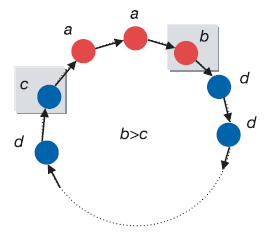
\includegraphics[width=0.5\textwidth]{natureGameSingle.png}
\end{tabular}
\caption{\label{fig:game} Mutant propagation game}
\end{figure}


More generalized, $W$ does not need to be stochastic, $w_{ij}>=0$. 
If the sum of all edges leaving a vertex is equal for all vertexes, then the graph will never suppress selection.
If the sum of all edges entering a vertex is equal for all vertexes, the graph never suppress drift.
If both then the graph is called a circulation.
     
To be able to point out insurable topologies, an extensive study of different graphs and how they behave has to be conducted. Regarding security, knowledge of how viruses spread and how to use graph structures to prevent malicious hackers from entering your network is important. Evolutionary dynamics, and the research of how mutant genes spread though out a population fits in to the model of security. 

Where the fixation probability determines the rate of evolution, which relies both on the size of the network and the evolution speed. A probability of 1 means that every node in the network eventually will be affected by the mutant.   
Isotherm graphs are a sub-graph of circulation. 

If $W$ is symmetric, or isotherm then the fixation probability is always \ref{eq:fixation}
isotherm means doubly stochastic, all rows and cols sum to 1. 
If a graph is one rooted, it has a fixation prob of $1/N$ regardless of $r$. If a graph has more then one root, its fixation probability is zero. 
Is it possible to find graphs with fixation probability that exceeds \ref{eq:fixation}? Is it possible to suppress drift and amplify selection?

And the selective difference is as we see amplified from $r$ to . i.e. a star act as an evolutionary amplifier,
 favoring advantageous mutants and inhibiting disadvantageous mutants, tilts towards selection and against drift.
 
 
 in certain graphs, star, funnel, metafunnel, if N is large enough, fixation probability for advantageous mutant converges to 1. Fixprob for disadvantageous converges to 0.
 
 
The same theory can be used to demonstrate how the aggregated security of a network is higher if the central node of a star structure is secured. 
If we assume that implemented security is 100$\%$ efficient, no threats will propagate beyond that node i.e total security for the network is increased. 
Scale-free networks have most of their connectivity clustered in a few vertices, i.e. they are potent selection amplifiers.







